\documentclass{article}

\usepackage[UTF8, scheme = plain]{ctex}
\usepackage{fancyhdr}
\usepackage{extramarks}
\usepackage{amsmath}
\usepackage{amsthm}
\usepackage{amsfonts}
\usepackage{tikz}
\usepackage[plain]{algorithm}
\usepackage{algpseudocode}
\usepackage{color}
\usepackage{listings}
\usepackage{fontspec}
\usepackage{float}

\newfontfamily\menlo{Menlo}
% \newfontfamily\menlo{Consolas}
\lstset{
    columns=fixed,       
    numbers=left,                                        % 在左侧显示行号
    numberstyle=\tiny\color{gray},                       % 设定行号格式
    frame=none,                                          % 不显示背景边框
    backgroundcolor=\color[RGB]{245,245,244},            % 设定背景颜色
    keywordstyle=\color[RGB]{40,40,255},                 % 设定关键字颜色
    numberstyle=\footnotesize\color{darkgray},           
    commentstyle=\it\color[RGB]{0,96,96},                % 设置代码注释的格式
    stringstyle=\rmfamily\slshape\color[RGB]{128,0,0},   % 设置字符串格式
    showstringspaces=true,                              % 不显示字符串中的空格
    numberstyle=\small\menlo,
    basicstyle=\small\menlo,
    breaklines=true,
}

% \lstset{
%     language=Octave,                % the language of the code
%     basicstyle=\footnotesize,           % the size of the fonts that are used for the code
%     numbers=left,                   % where to put the line-numbers
%     numberstyle=\tiny\color{gray},  % the style that is used for the line-numbers
%     stepnumber=1,                   % the step between two line-numbers. If it's 1, each line 
%                                     % will be numbered
%     numbersep=5pt,                  % how far the line-numbers are from the code
%     backgroundcolor=\color{white},      % choose the background color. You must add \usepackage{color}
%     showspaces=false,               % show spaces adding particular underscores
%     showstringspaces=false,         % underline spaces within strings
%     showtabs=false,                 % show tabs within strings adding particular underscores
%     frame=single,                   % adds a frame around the code
%     rulecolor=\color{black},        % if not set, the frame-color may be changed on line-breaks within not-black text (e.g. commens (green here))
%     tabsize=2,                      % sets default tabsize to 2 spaces
%     captionpos=b,                   % sets the caption-position to bottom
%     breaklines=true,                % sets automatic line breaking
%     breakatwhitespace=false,        % sets if automatic breaks should only happen at whitespace
%     title=\lstname,                 % show the filename of files included with \lstinputlisting;
%                                     % also try caption instead of title
%     keywordstyle=\color{blue},          % keyword style
%     commentstyle=\color{dkgreen},       % comment style
%     stringstyle=\color{mauve},         % string literal style
%     escapeinside={\%*}{*)},            % if you want to add LaTeX within your code
%     morekeywords={*,...}               % if you want to add more keywords to the set
% }

\usetikzlibrary{automata,positioning}

%
% Basic Document Settings
%
%%% page layout
\topmargin=-0.45in
\evensidemargin=0in
\oddsidemargin=0in
\textwidth=6.5in
\textheight=9.0in
\headsep=0.25in

\linespread{1.1}    %%% line spacing

\definecolor{ustcblue}{cmyk}{1,0.8,0,0}

\pagestyle{fancy}
\lhead{\hmwkAuthorName}
\chead{\hmwkClass\ (\hmwkClassInstructor): \hmwkTitle}
\rhead{}
\lfoot{}
\cfoot{\thepage}

\renewcommand\headrulewidth{0.4pt}
\renewcommand\footrulewidth{0.4pt}

\setlength\parindent{0pt}

%
% Create Problem Sections
%

\newcommand{\enterProblemHeader}[1]{
    \nobreak\extramarks{}{Problem \arabic{#1} continued on next page\ldots}\nobreak{}
    \nobreak\extramarks{Problem \arabic{#1} (continued)}{Problem \arabic{#1} continued on next page\ldots}\nobreak{}
}

\newcommand{\exitProblemHeader}[1]{
    \nobreak\extramarks{Problem \arabic{#1} (continued)}{Problem \arabic{#1} continued on next page\ldots}\nobreak{}
    \stepcounter{#1}
    \nobreak\extramarks{Problem \arabic{#1}}{}\nobreak{}
}

\setcounter{secnumdepth}{0}
\newcounter{partCounter}
\newcounter{homeworkProblemCounter}
\setcounter{homeworkProblemCounter}{1}
\nobreak\extramarks{Problem \arabic{homeworkProblemCounter}}{}\nobreak{}

%
% Homework Problem Environment
%
% This environment takes an optional argument. When given, it will adjust the
% problem counter. This is useful for when the problems given for your
% assignment aren't sequential. See the last 3 problems of this template for an
% example.
%
\newenvironment{homeworkProblem}[1][-1]{
    \ifnum#1>0
        \setcounter{homeworkProblemCounter}{#1}
    \fi
    \subsection{Exercise \arabic{homeworkProblemCounter}}
    \setcounter{partCounter}{1}
    \enterProblemHeader{homeworkProblemCounter}
}{
    \exitProblemHeader{homeworkProblemCounter}
}

%
% Homework Details
%   - Title
%   - Due date
%   - Class
%   - Section/Time
%   - Instructor
%   - Author
%

\newcommand{\hmwkTitle}{Homework\ \#2}
\newcommand{\hmwkDueDate}{\today}
\newcommand{\hmwkClass}{Geodynamics}
\newcommand{\hmwkClassInstructor}{Professor W. Len}
\newcommand{\hmwkAuthorName}{\textbf{Jintao Li}}
\newcommand{\hmwkAuthorID}{\textbf{SA20007037}}
\newcommand{\hmwkAuthoremail}{\textbf{E-mail: lijintao@mail.ustc.edu.cn}}

%
% Title Page
%

% \title{
%     \vspace{2in}
%     \textbf{\hmwkClass:\ \hmwkTitle}\\
%     \normalsize\vspace{0.2in}\large{\hmwkDueDate}\\
%     \vspace{0.2in}\large{\textit{\hmwkClassInstructor}}
%     \vspace{3in}
% }

% \author{\hmwkAuthorName \\
% \hmwkAuthorID}
% \date{}

\renewcommand{\part}[1]{\textbf{ \\ (\alph{partCounter})  }\stepcounter{partCounter} }

%
% Various Helper Commands
%

% Useful for algorithms
\newcommand{\alg}[1]{\textsc{\bfseries \footnotesize #1}}

% For derivatives
\newcommand{\deriv}[1]{\frac{\mathrm{d}}{\mathrm{d}x} (#1)}

% For partial derivatives
\newcommand{\pderiv}[2]{\frac{\partial}{\partial #1} (#2)}

% Integral dx
\newcommand{\dx}{\mathrm{d}x}

% Alias for the Solution section header
\newcommand{\solution}{\textbf{\large \\ Solution: \\}}

% Probability commands: Expectation, Variance, Covariance, Bias
\newcommand{\E}{\mathrm{E}}
\newcommand{\Var}{\mathrm{Var}}
\newcommand{\Cov}{\mathrm{Cov}}
\newcommand{\Bias}{\mathrm{Bias}}

%
\newcommand{\mb}[1]{\mathbf{#1}}

\begin{document}

\begin{titlepage}

\begin{center}

\textcolor{ustcblue}{
\includegraphics[width=0.4\textwidth]{../hw1/ustc_logo_fig.pdf} \\ [1cm]}
% Title
{ \Huge \bfseries \hmwkClass\ \hmwkTitle}\\[1cm]

\large \textbf{\hmwkClassInstructor} \\ [5cm]

\large \hmwkAuthorName \\ [0.25cm]
\large \hmwkAuthorID \\ [0.25cm]
\large \hmwkAuthoremail
\vfill
% Bottom of the page
{\large April 06, 2021}

\end{center}

\end{titlepage}

\begin{center}
\section{Chapter 1: Stress and Strain}
\end{center}

\subsection{Note: }
\textbf{The code was attached with this file, the python file (*.py) is 
used to calculate the results and the shell file (*.sh) is used 
to plot figures.} \\


\begin{homeworkProblem}[1]
Download the CRUST 1.0 crust thickness data. According to isostasy, compute 
the global isostatic topography.

\solution

First, we downloaded the CRUST 1.0 crust thickness data from website: 
\textcolor{blue}{https://igppweb.ucsd.edu/~gabi/crust1.html}. Then, 
we extracted the file: \textbf{crust1.0.tar.gz}, compiled the fortran file:
\textbf{getCN1xyz.f} using gfortran: \textbf{gfortran getCN1xyz.f -o getCN1xyz}. \\

After running getCN1xyz program, we obtained the boundary depth, density, thickness,
p-wave and s-wave velocity of each layer, crust thickness (2~8 layers) and 
sedimentary thickness (3~5 layers). We divided the global crust to two type: 
continent and ocean by a threshold thickness (12 km) and then calculated the 
evelation by the following equtions:

\begin{equation}
E_{continent} = h_{continental\_crust}-\frac{\rho_{c}}{\rho_{m}} 
h_{continental\_crust}
=h_{continental\_crust} \left(1-\frac{\rho_{continental\_crust}}{\rho_{mantle}}\right)
\end{equation}

\begin{equation}
E_{ocean}=\frac{\left(\rho_{mantle}-\rho_{continental\_crust}\right)}
{\left(\rho_{mantle}-\rho_{water}\right)} h_{continental\_crust}-
\frac{\left(\rho_{mantle}-\rho_{ocean_curst}\right)}
{\left(\rho_{mantle}-\rho_{water}\right)} h_{ocean\_curst}
\end{equation}

The total thickness of 1-8 layers is represented continental 
crust thickness. And it is already stored in file \textbf{crsthk.xyz}. 
For ocean, the continental crust thickness and it's density is necessary, 
and we simply set them as the average value: $35 km$, $2800 kg/m^3$.
Finally, we plotted the global isostatic topography by GMT.\\


\textbf{The figures}
\begin{figure}[H]
    \centering
    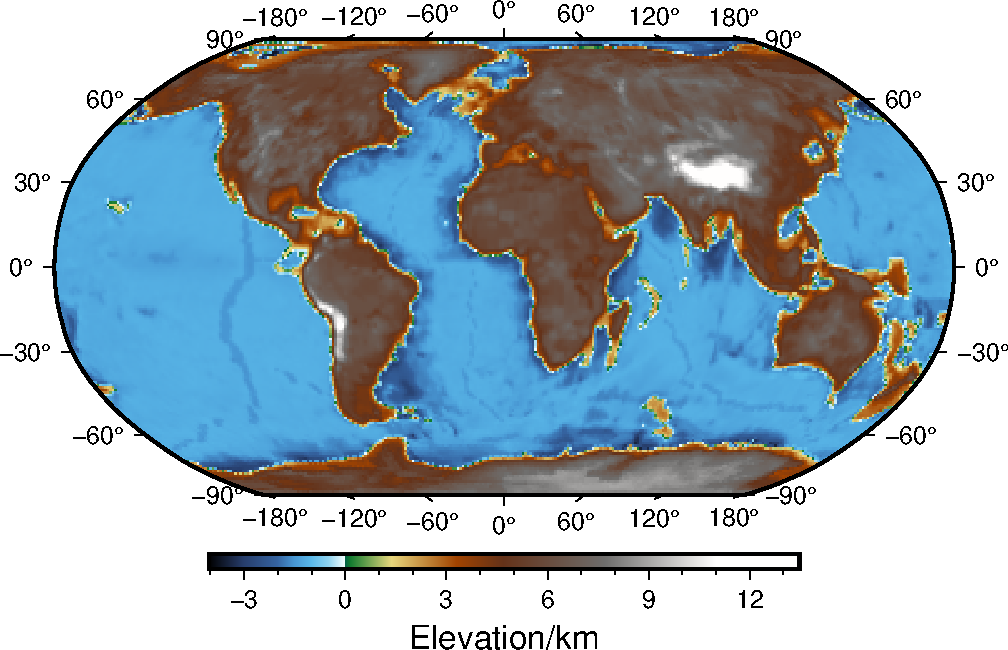
\includegraphics[width=6in, keepaspectratio]{elevation.pdf}
    \label{fig:elevation}
\end{figure}

\end{homeworkProblem}

\pagebreak


\begin{homeworkProblem}[2]
Compute and plot the difference between the isostatic topography and the 
actual topography (ETOPO1). Discuss your results.

\solution

We need not to download ETOPO1 topography data, beacause from the handbook of 
crust1.0, \textit{Bathymetry and topography is that of ETOPO1} and \textit{
From the ETOPO1 files, we derived topography, bathymetry and ice thickness in 
our new model by binning and averaging the ETOPO1 data in 1-degree cells.} 
So, we leverage the lower boundary of water to represent the ETOPO1 topography.
Finally, we plotted the difference by GMT.\\

\textbf{Discuss:}\\

The result shows that there is a larger difference in continent than in ocean.
Beacause the formula used to calculate ocean topography is more \textbf{realistic} 
than the first which is used in continent (according to the slids provided by 
Professor Len). And the effect of water and ocean crust is ignored in the formula 
used in continent and it assumes that continent is just floating on the mantle. 
So the difference of continent is larger than ocean's.\\


\textbf{The figure}
\begin{figure}[H]
    \centering
    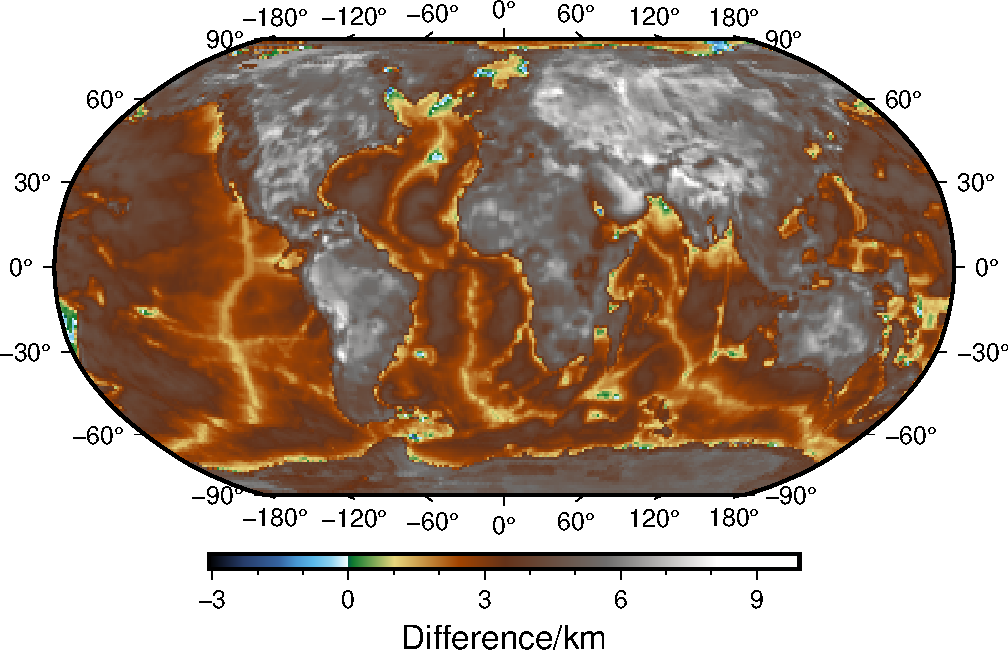
\includegraphics[width=6in, keepaspectratio]{diffence.pdf}
    \label{fig:difference}
\end{figure}
    
\end{homeworkProblem}

\pagebreak

\begin{homeworkProblem}[3]
Choose a specific region, and do the same thing in 1. and 2. for this region.
Discuss your results.

\solution

Beacause to calculate results of a specific region, we use the same data and 
formula. So, we don't calculate again but just change the parameter -R 
when plotting by GMT. We choose the South America as an example. \\ 

\textbf{Discuss:} \\

The situation is similar to the second question. So we don't repeat it again \\

\textbf{The figure}
\begin{figure}[H]
    \centering
    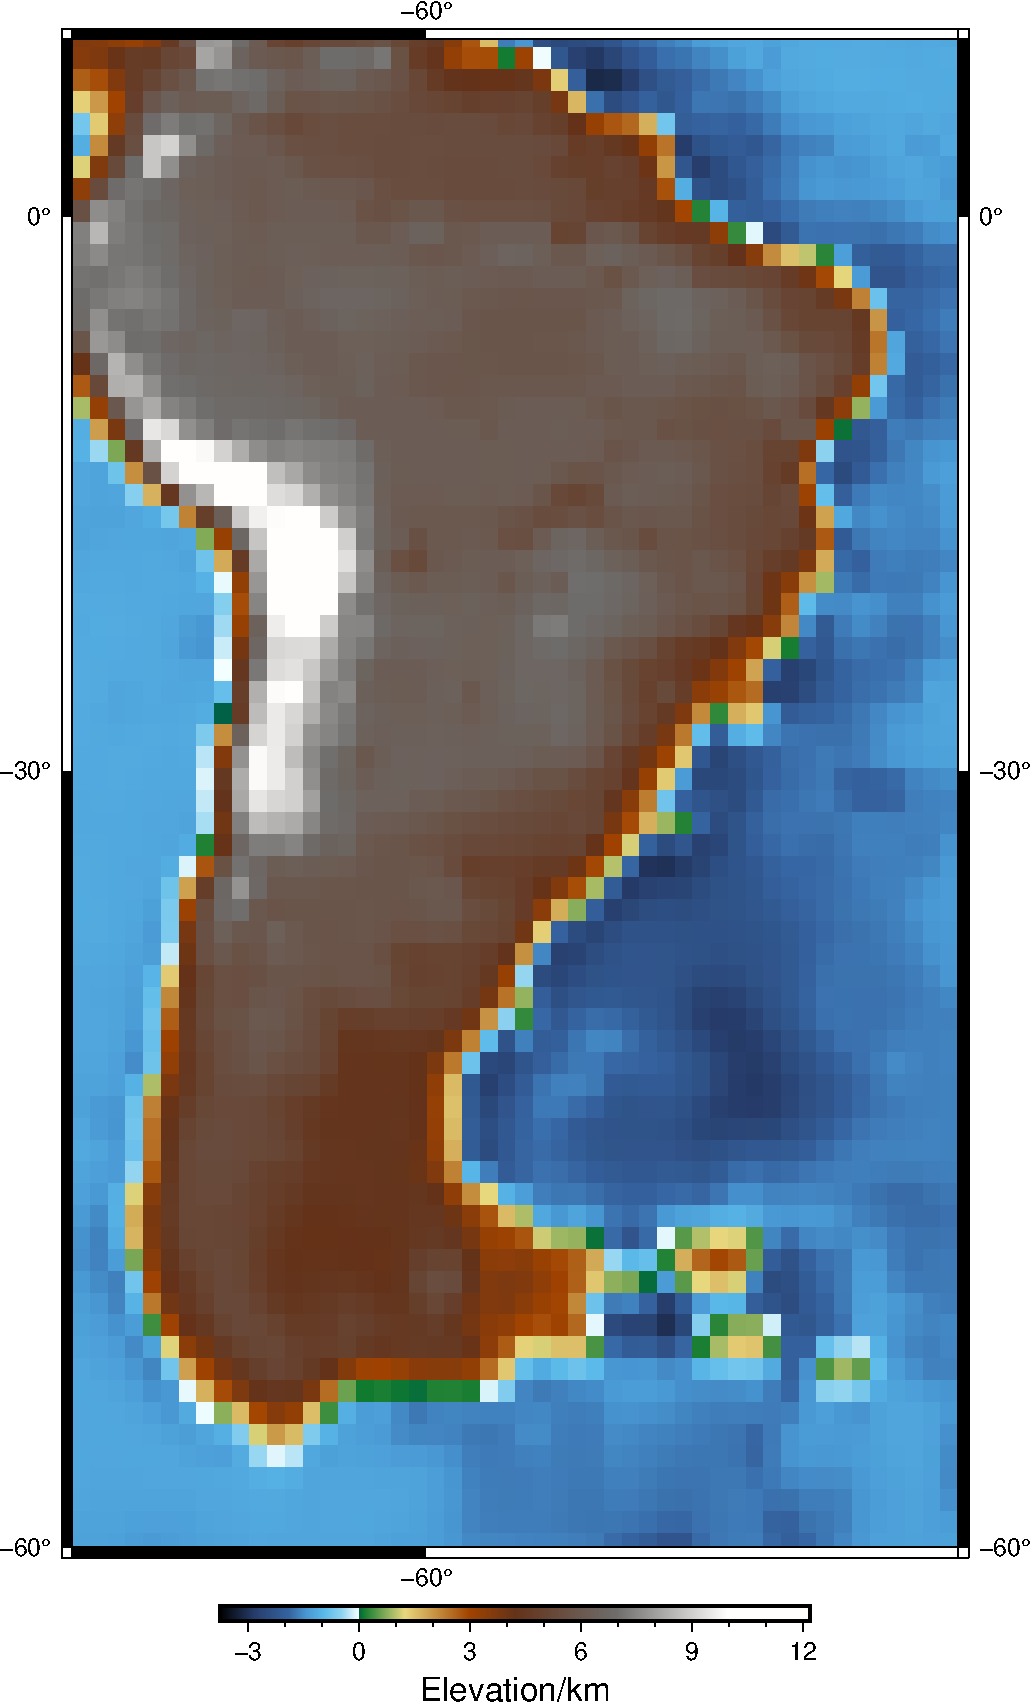
\includegraphics[width=5in, keepaspectratio]{e_local.pdf}
    \label{fig:e_local}
\end{figure}

\begin{figure}[H]
    \centering
    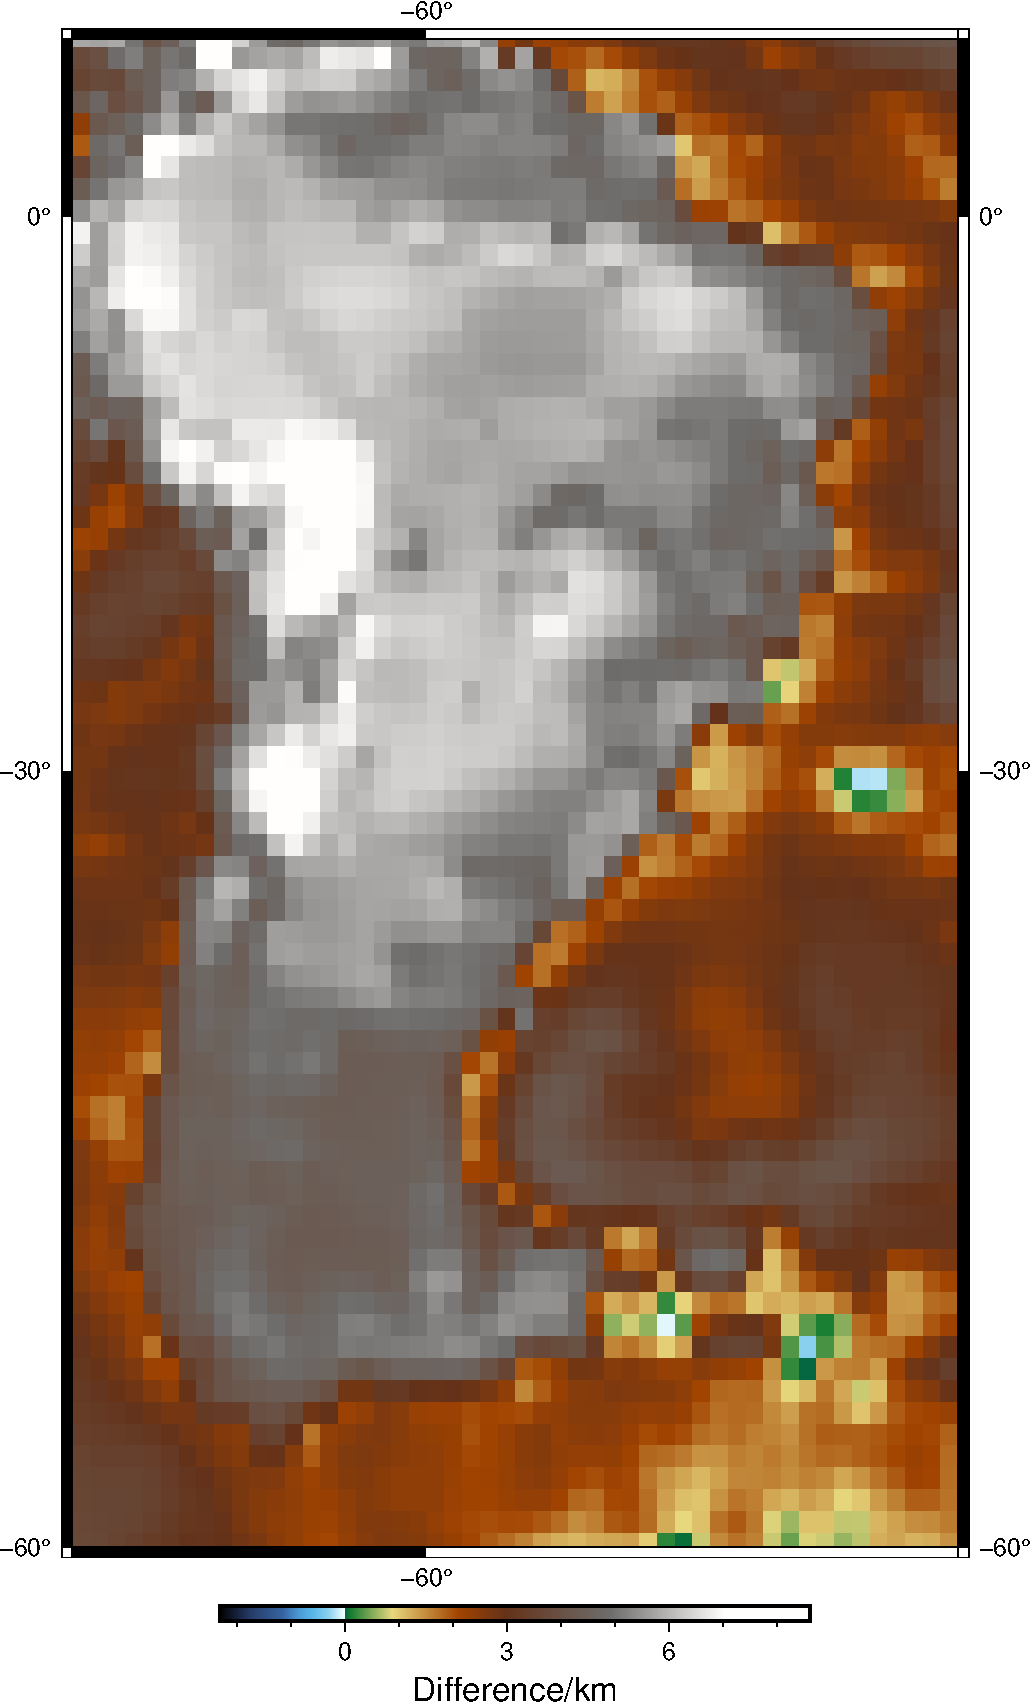
\includegraphics[width=5in, keepaspectratio]{d_local.pdf}
    \label{fig:d_local}
\end{figure}


\end{homeworkProblem}


\end{document}
